\documentclass[11pt,a4paper]{scrartcl}

%% ── Encoding & Language ─────────────────────────────────────────────────────
\usepackage[T1]{fontenc}
\usepackage[utf8]{inputenc}
\usepackage[english]{babel}

%% ── Fonts ────────────────────────────────────────────────────────────────────
\usepackage{lmodern}
\usepackage{microtype}

%% ── Page Layout ──────────────────────────────────────────────────────────────
\usepackage[
  a4paper,
  top=22mm, bottom=25mm,
  left=22mm, right=22mm,
  headheight=14pt
]{geometry}

%% ── Colours ──────────────────────────────────────────────────────────────────
\usepackage[table,dvipsnames]{xcolor}
\definecolor{NavyDeep}{HTML}{1A2E4A}
\definecolor{TealAccent}{HTML}{2A7F8A}
\definecolor{WarmSand}{HTML}{F5F0E8}
\definecolor{CrimsonAlert}{HTML}{C0392B}
\definecolor{SlateLight}{HTML}{ECF0F3}
\definecolor{SlateRule}{HTML}{BDC8D4}
\definecolor{TextMain}{HTML}{1C2833}
\definecolor{TextMuted}{HTML}{5D6D7E}
\definecolor{SuccessGreen}{HTML}{1E8449}
\definecolor{AmberWarn}{HTML}{B7770D}

%% ── Mathematics ──────────────────────────────────────────────────────────────
\usepackage{amsmath}
\usepackage{amssymb}

%% ── Tables ───────────────────────────────────────────────────────────────────
\usepackage{booktabs}
\usepackage{tabularx}
\usepackage{array}
\usepackage{colortbl}
\usepackage{multirow}
\usepackage{makecell}

%% ── Graphics & Boxes ─────────────────────────────────────────────────────────
\usepackage{graphicx}
\usepackage[most]{tcolorbox}
\usepackage{tikz}
\usetikzlibrary{positioning,calc,shapes.geometric,decorations.pathmorphing,backgrounds,patterns}

%% ── Lists ────────────────────────────────────────────────────────────────────
\usepackage{enumitem}

%% ── Header / Footer ──────────────────────────────────────────────────────────
\usepackage{fancyhdr}
\usepackage{lastpage}

%% ── Misc ─────────────────────────────────────────────────────────────────────
\usepackage{fontawesome5}
\usepackage{calc}
\usepackage{parskip}
\usepackage{dashrule}
\usepackage{ifthen}
\usepackage{ragged2e}

%% ── KOMA tweaks ──────────────────────────────────────────────────────────────
\setkomafont{disposition}{\normalfont\bfseries\color{NavyDeep}}

%% ── Page Style ───────────────────────────────────────────────────────────────
\pagestyle{fancy}
\fancyhf{}
\renewcommand{\headrulewidth}{0pt}
\fancyhead[L]{%
  
\begin{tikzpicture}[remember picture, overlay]
    \fill[NavyDeep] (0,0) rectangle (\paperwidth, 0.65cm);
  \end{tikzpicture}%
  \raisebox{0.05cm}{\textcolor{white}{\footnotesize\textbf{MERIDIAN ONCOLOGY CENTRE} \quad\textbar\quad Chemotherapy \& Radiation Protocol Reference}}%
}
\fancyfoot[C]{%
  \textcolor{TextMuted}{\scriptsize
    \textbf{SPECIMEN — FOR TRAINING PURPOSES ONLY} \quad\textbar\quad
    Page~\thepage\ of~\pageref{LastPage} \quad\textbar\quad
    Protocol ID: MOC-2025-NSCLC-004
  }%
}
\fancyfoot[R]{%
  
\begin{tikzpicture}[remember picture, overlay]
    \fill[NavyDeep] (0,0) rectangle (3.2cm, 0.4cm);
    \node[white, font=\tiny\bfseries] at (1.6cm, 0.2cm) {CONFIDENTIAL};
  \end{tikzpicture}%
}

%% ── SPECIMEN watermark ────────────────────────────────────────────────────────
\usepackage{eso-pic}
\AddToShipoutPictureBG{%
  \begin{tikzpicture}[remember picture, overlay]
    \node[
      rotate=45,
      font=\fontsize{72}{72}\selectfont\bfseries,
      text=black!10,
      at=(current page.center)
    ] {SPECIMEN};
  \end{tikzpicture}%
}

%% ── tcolorbox styles ─────────────────────────────────────────────────────────
\tcbuselibrary{breakable,skins,theorems}

\tcbset{
  protocolbox/.style={
    enhanced,
    breakable,
    colback=SlateLight,
    colframe=NavyDeep,
    coltitle=white,
    fonttitle=\bfseries\small,
    attach boxed title to top left={yshift=-2mm, xshift=5mm},
    boxed title style={
      colback=NavyDeep,
      colframe=NavyDeep,
      rounded corners,
      interior style={fill=NavyDeep},
    },
    arc=3pt,
    boxrule=0.8pt,
    top=6pt, bottom=6pt, left=7pt, right=7pt,
  },
  warnbox/.style={
    enhanced,
    colback=CrimsonAlert!6,
    colframe=CrimsonAlert,
    coltitle=white,
    fonttitle=\bfseries\small,
    attach boxed title to top left={yshift=-2mm, xshift=5mm},
    boxed title style={colback=CrimsonAlert, colframe=CrimsonAlert, rounded corners},
    arc=3pt,
    boxrule=0.8pt,
    top=6pt, bottom=6pt, left=7pt, right=7pt,
  },
  infobox/.style={
    enhanced,
    colback=TealAccent!8,
    colframe=TealAccent,
    coltitle=white,
    fonttitle=\bfseries\small,
    attach boxed title to top left={yshift=-2mm, xshift=5mm},
    boxed title style={colback=TealAccent, colframe=TealAccent, rounded corners},
    arc=3pt,
    boxrule=0.8pt,
    top=6pt, bottom=6pt, left=7pt, right=7pt,
  },
  successbox/.style={
    enhanced,
    colback=SuccessGreen!6,
    colframe=SuccessGreen,
    coltitle=white,
    fonttitle=\bfseries\small,
    attach boxed title to top left={yshift=-2mm, xshift=5mm},
    boxed title style={colback=SuccessGreen, colframe=SuccessGreen, rounded corners},
    arc=3pt,
    boxrule=0.8pt,
    top=6pt, bottom=6pt, left=7pt, right=7pt,
  },
}

%% ── Custom commands ──────────────────────────────────────────────────────────
\newcommand{\sectionrule}{%
  \par\vspace{2pt}\noindent%
  {\color{TealAccent}\rule{\linewidth}{1.5pt}}\par\par%
  \vspace{4pt}%
}

\newcommand{\subsectionrule}{%
  \par\noindent%
  \vspace{1pt}%
  {\color{SlateRule}\rule{\linewidth}{0.6pt}}\par%
  \vspace{3pt}%
}

\newcommand{\badge}[2]{%
  \begin{tikzpicture}[baseline=(b.base)]
    \node[
      fill=#1,
      rounded corners=3pt,
      inner xsep=4pt, inner ysep=2.5pt,
      font=\tiny\bfseries,
      text=white
    ] (b) {#2};
  \end{tikzpicture}%
}

\newcommand{\cyclebullet}[1]{%
  \begin{tikzpicture}[baseline=(c.base)]
    \node[
      circle,
      fill=TealAccent,
      inner sep=2pt,
      font=\tiny\bfseries,
      text=white
    ] (c) {#1};
  \end{tikzpicture}%
}

\newcommand{\drugname}[1]{\textbf{\textcolor{NavyDeep}{#1}}}
\newcommand{\dose}[1]{\texttt{\textcolor{TealAccent}{#1}}}
\newcommand{\alert}[1]{\textbf{\textcolor{CrimsonAlert}{#1}}}
\newcommand{\ok}[1]{\textbf{\textcolor{SuccessGreen}{#1}}}
\newcommand{\field}[1]{\underline{\hspace{#1}}}

%% ── Column types ─────────────────────────────────────────────────────────────
\newcolumntype{L}[1]{>{\RaggedRight\arraybackslash}p{#1}}
\newcolumntype{C}[1]{>{\Centering\arraybackslash}p{#1}}

%% ─────────────────────────────────────────────────────────────────────────────
\begin{document}
%% ─────────────────────────────────────────────────────────────────────────────

%% ═══════════════════════════════════════════════════════════════════════════
%%  TITLE BLOCK
%% ═══════════════════════════════════════════════════════════════════════════
\thispagestyle{fancy}
\vspace*{4mm}

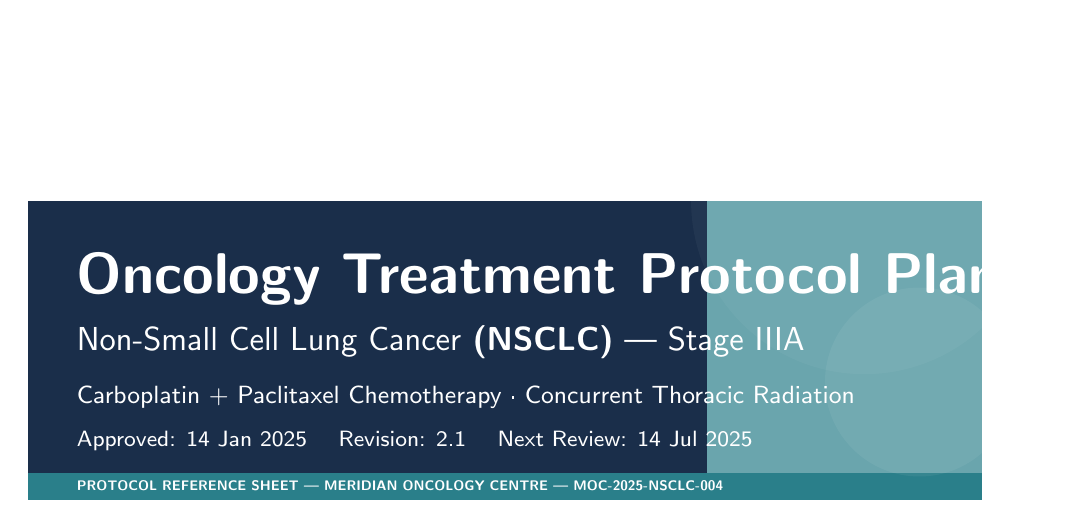
\begin{tikzpicture}
  \fill[NavyDeep] (0,0) rectangle (\linewidth, 3.8cm);
  \fill[TealAccent] (0,0) rectangle (\linewidth, 0.35cm);
  %% accent bar
  \fill[TealAccent!70] (\linewidth - 3.5cm, 0.35cm) rectangle (\linewidth, 3.8cm);
  %% decorative circles
  \fill[white, opacity=0.04] (\linewidth - 1.5cm, 3.8cm) circle (2.2cm);
  \fill[white, opacity=0.06] (\linewidth - 0.8cm, 1.5cm) circle (1.2cm);
  %% text
  \node[white, font=\tiny\bfseries\sffamily, anchor=west]
    at (0.5cm, 0.18cm) {PROTOCOL REFERENCE SHEET — MERIDIAN ONCOLOGY CENTRE — MOC-2025-NSCLC-004};
  \node[white, font=\fontsize{22}{26}\selectfont\bfseries\sffamily, anchor=west]
    at (0.5cm, 2.8cm) {Oncology Treatment Protocol Plan};
  \node[white!80, font=\large\sffamily, anchor=west]
    at (0.5cm, 2.0cm) {Non-Small Cell Lung Cancer \textbf{(NSCLC)} — Stage IIIA};
  \node[white!70, font=\small\sffamily, anchor=west]
    at (0.5cm, 1.3cm) {Carboplatin + Paclitaxel Chemotherapy \textperiodcentered{} Concurrent Thoracic Radiation};
  \node[white!60, font=\footnotesize\sffamily, anchor=west]
    at (0.5cm, 0.75cm) {Approved: 14 Jan 2025 \quad Revision: 2.1 \quad Next Review: 14 Jul 2025};
\end{tikzpicture}

\vspace{5mm}

%% ═══════════════════════════════════════════════════════════════════════════
%%  PATIENT & TEAM INFORMATION (two-column minipage)
%% ═══════════════════════════════════════════════════════════════════════════

\noindent
\begin{minipage}[t]{0.485\linewidth}
  \begin{tcolorbox}[
    protocolbox,
    title={\faUser\quad Patient Information},
    breakable=false
  ]
    \footnotesize
    \begin{tabular}{@{}lp{4.2cm}@{}}
      \textbf{Name:}       & Eleanor Margaret Osei \\[2pt]
      \textbf{DOB:}        & 17 March 1963 \\[2pt]
      \textbf{MRN:}        & MOC-2025-08841 \\[2pt]
      \textbf{Sex:}        & Female \\[2pt]
      \textbf{Weight:}     & 68 kg \quad\textbar\quad Height: 164 cm \\[2pt]
      \textbf{BSA:}        & 1.74 m\textsuperscript{2} \quad\textbf{(Mosteller)} \\[2pt]
      \textbf{ECOG PS:}    & \badge{TealAccent}{1} \\[2pt]
      \textbf{Allergies:}  & \alert{Sulfonamides} \\[2pt]
      \textbf{Diagnosis:}  & NSCLC, Adenocarcinoma \\[2pt]
      \textbf{Stage:}      & IIIA (T3N2M0) \\[2pt]
      \textbf{Biomarkers:} & EGFR\textsuperscript{--}, ALK\textsuperscript{--}, PD-L1: 35\% \\[2pt]
    \end{tabular}
  \end{tcolorbox}
\end{minipage}%
\hfill
\begin{minipage}[t]{0.485\linewidth}
  \begin{tcolorbox}[
    infobox,
    title={\faUserMd\quad Multidisciplinary Team},
    breakable=false
  ]
    \footnotesize
    \begin{tabular}{@{}lp{4.2cm}@{}}
      \textbf{Medical Oncologist:}   & Dr. Samuel Adeyemi, MD \\[2pt]
      \textbf{Radiation Oncologist:} & Dr. Priya Nair, MD, FRCR \\[2pt]
      \textbf{Pulmonologist:}        & Dr. Thomas Bergmann \\[2pt]
      \textbf{Pharmacist:}           & Claire Fontaine, PharmD \\[2pt]
      \textbf{Oncology Nurse:}       & Beatrice Okafor, RN \\[2pt]
      \textbf{MDT Date:}             & 10 Jan 2025 \\[2pt]
      \textbf{Institution:}          & Meridian Oncology Centre \\[2pt]
      \textbf{Department:}           & Thoracic Oncology Unit \\[2pt]
      \textbf{Contact:}              & \faPhone\ +44\,(0)20\,7946\,0871 \\[2pt]
      \textbf{Email:}                & thoracic@meridian-onc.nhs.uk \\[2pt]
    \end{tabular}
  \end{tcolorbox}
\end{minipage}

\par
\vspace{4mm}

%% ═══════════════════════════════════════════════════════════════════════════
%%  TREATMENT INTENT & OVERVIEW
%% ═══════════════════════════════════════════════════════════════════════════

\noindent{\large\bfseries\color{NavyDeep}\faClipboardList\enspace Treatment Intent \& Overview}
\sectionrule

\noindent
\begin{minipage}[t]{0.30\linewidth}
  \begin{tcolorbox}[
    enhanced,
    colback=NavyDeep,
    colframe=NavyDeep,
    arc=4pt,
    boxrule=0pt,
    top=8pt, bottom=8pt, left=8pt, right=8pt
  ]
    \centering
    \textcolor{TealAccent}{\small\bfseries INTENT}\\[4pt]
    \textcolor{white}{\Large\bfseries Curative}\\[4pt]
    \textcolor{white!70}{\tiny Concurrent CRT}
  \end{tcolorbox}
\end{minipage}%
\hspace{2mm}
\begin{minipage}[t]{0.30\linewidth}
  \begin{tcolorbox}[
    enhanced,
    colback=TealAccent,
    colframe=TealAccent,
    arc=4pt,
    boxrule=0pt,
    top=8pt, bottom=8pt, left=8pt, right=8pt
  ]
    \centering
    \textcolor{white!80}{\small\bfseries CYCLES}\\[4pt]
    \textcolor{white}{\Large\bfseries 6 Cycles}\\[4pt]
    \textcolor{white!70}{\tiny 21-day intervals}
  \end{tcolorbox}
\end{minipage}%
\hspace{2mm}
\begin{minipage}[t]{0.30\linewidth}
  \begin{tcolorbox}[
    enhanced,
    colback=NavyDeep!80,
    colframe=NavyDeep!80,
    arc=4pt,
    boxrule=0pt,
    top=8pt, bottom=8pt, left=8pt, right=8pt
  ]
    \centering
    \textcolor{TealAccent!80}{\small\bfseries TOTAL DURATION}\\[4pt]
    \textcolor{white}{\Large\bfseries 18 Weeks}\\[4pt]
    \textcolor{white!70}{\tiny Chemo + RT}
  \end{tcolorbox}
\end{minipage}

\par
\vspace{4mm}

%% ═══════════════════════════════════════════════════════════════════════════
%%  CHEMOTHERAPY DOSING SCHEDULE
%% ═══════════════════════════════════════════════════════════════════════════

\noindent{\large\bfseries\color{NavyDeep}\faCapsules\enspace Chemotherapy Dosing Schedule}
\sectionrule

\begin{tcolorbox}[protocolbox, title={\faCapsules\quad Regimen: Carboplatin + Paclitaxel (CarboTax)}]

\footnotesize

\textbf{\textcolor{NavyDeep}{Protocol:}} Carboplatin AUC 6 + Paclitaxel 200\,mg/m\textsuperscript{2} every 21 days (Q21D) $\times$ 6 cycles.
Concurrent thoracic radiotherapy during Cycles 1 and 2.

\vspace{5pt}

\noindent\textbf{\textcolor{NavyDeep}{Calculated Doses} (BSA = 1.74\,m\textsuperscript{2}; GFR = 82\,mL/min):}

\vspace{3pt}

\rowcolors{2}{SlateLight}{white}
\begin{tabularx}{\linewidth}{@{} l C{2.0cm} C{2.2cm} C{2.0cm} C{2.8cm} @{}}
  \toprule
  \rowcolor{NavyDeep}
  \textcolor{white}{\bfseries Drug} &
  \textcolor{white}{\bfseries Dose/m\textsuperscript{2}} &
  \textcolor{white}{\bfseries Calc.\ Dose} &
  \textcolor{white}{\bfseries Route} &
  \textcolor{white}{\bfseries Infusion Duration} \\
  \midrule
  \drugname{Paclitaxel}   & \dose{200\,mg/m\textsuperscript{2}} & \dose{348\,mg}  & IV & 3 hours \\
  \drugname{Carboplatin}  & \dose{AUC\,6}                       & \dose{528\,mg}  & IV & 30 minutes \\
  \drugname{Dexamethasone (pre-med)} & \dose{20\,mg fixed}  & \dose{20\,mg}   & IV & 15 minutes \\
  \drugname{Diphenhydramine (pre-med)} & \dose{50\,mg fixed} & \dose{50\,mg}  & IV & 15 minutes \\
  \drugname{Ranitidine (pre-med)} & \dose{50\,mg fixed}     & \dose{50\,mg}   & IV & 15 minutes \\
  \bottomrule
\end{tabularx}

\vspace{6pt}

\textbf{\textcolor{NavyDeep}{Carboplatin AUC Calculation (Calvert):}}
\[
  \text{Dose\,(mg)} = \text{AUC} \times \bigl(\text{GFR} + 25\bigr) = 6 \times (82 + 25) = \mathbf{642\,mg}
\]
\textit{\textcolor{TextMuted}{\footnotesize Note: Capped at 1,000\,mg maximum per institutional policy. Actual dispensed dose: 642\,mg.}}

\end{tcolorbox}

\par
\vspace{3mm}

%% ─── Cycle Schedule Table ──────────────────────────────────────────────────
\noindent{\bfseries\color{NavyDeep}\faCalendar\enspace Cycle Calendar}
\subsectionrule

\footnotesize
\rowcolors{2}{SlateLight}{white}
\begin{tabularx}{\linewidth}{@{} C{0.9cm} C{2.2cm} C{2.4cm} C{1.8cm} C{1.8cm} L{4.5cm} @{}}
  \toprule
  \rowcolor{NavyDeep}
  \textcolor{white}{\bfseries Cycle} &
  \textcolor{white}{\bfseries Start Date} &
  \textcolor{white}{\bfseries Chemo Day} &
  \textcolor{white}{\bfseries Paclitaxel} &
  \textcolor{white}{\bfseries Carboplatin} &
  \textcolor{white}{\bfseries Notes} \\
  \midrule
  \cyclebullet{1} & 20 Jan 2025 & Day 1 & 348\,mg & 642\,mg & Concurrent RT (wk 1--2) \\
  \cyclebullet{2} & 10 Feb 2025 & Day 22 & 348\,mg & 642\,mg & Concurrent RT (wk 3--6) \\
  \cyclebullet{3} & 03 Mar 2025 & Day 43 & 348\,mg & 642\,mg & Post-RT consolidation \\
  \cyclebullet{4} & 24 Mar 2025 & Day 64 & 348\,mg & 642\,mg & Restaging CT after Cycle 4 \\
  \cyclebullet{5} & 14 Apr 2025 & Day 85 & 348\,mg & 642\,mg & Dose reduce if Grade\,\(\geq\)3 tox \\
  \cyclebullet{6} & 05 May 2025 & Day 106 & 348\,mg & 642\,mg & Final cycle; end-of-tx imaging \\
  \bottomrule
\end{tabularx}

\par
\vspace{4mm}

%% ─── Pre-medication Protocol ───────────────────────────────────────────────
\noindent
\begin{minipage}[t]{0.475\linewidth}
  \begin{tcolorbox}[infobox, title={\faSyringe\quad Pre-medication Protocol}, breakable=false]
    \footnotesize
    \begin{enumerate}[leftmargin=1.2em, label=\textbf{\arabic*.}, itemsep=2pt]
      \item \drugname{Dexamethasone} 20\,mg IV, 30\,min pre-Paclitaxel
      \item \drugname{Diphenhydramine} 50\,mg IV, 30\,min pre-Paclitaxel
      \item \drugname{Ranitidine} 50\,mg IV, 30\,min pre-Paclitaxel
      \item \drugname{Ondansetron} 8\,mg IV, 30\,min pre-chemo
      \item \drugname{Dexamethasone} 8\,mg PO BD $\times$ 3 days post-chemo
      \item \drugname{Ondansetron} 8\,mg PO TDS $\times$ 5 days post-chemo
    \end{enumerate}
  \end{tcolorbox}
\end{minipage}%
\hfill
\begin{minipage}[t]{0.495\linewidth}
  \begin{tcolorbox}[warnbox, title={\faExclamationTriangle\quad Dose Modification Triggers}, breakable=false]
    \footnotesize
    \begin{tabular}{@{} l p{4.6cm} @{}}
      \toprule
      \textbf{Toxicity} & \textbf{Action} \\
      \midrule
      ANC\,$<$\,1.5\,\(\times\)10\textsuperscript{9}/L & Delay cycle 1 week \\
      Plt\,$<$\,100\,\(\times\)10\textsuperscript{9}/L & Delay; reduce Carboplatin 25\% \\
      Creatinine clearance\,$<$\,45 & Reduce Carboplatin to AUC 5 \\
      Grade\,\(\geq\)2 neuropathy & Reduce Paclitaxel 20\% \\
      Grade\,3 nausea/vomiting & Add Aprepitant 125\,mg D1 \\
    \end{tabular}
  \end{tcolorbox}
\end{minipage}

\par
\vspace{5mm}

%% ═══════════════════════════════════════════════════════════════════════════
%%  RADIATION PROTOCOL
%% ═══════════════════════════════════════════════════════════════════════════

\noindent{\large\bfseries\color{NavyDeep}\faRadiation\enspace Radiation Therapy Protocol}
\sectionrule

\noindent
\begin{minipage}[t]{0.475\linewidth}
  \begin{tcolorbox}[protocolbox, title={\faRulerCombined\quad Treatment Parameters}, breakable=false]
    \footnotesize
    \begin{tabular}{@{} l p{4.5cm} @{}}
      \textbf{Modality:}        & External Beam RT (EBRT) \\[2pt]
      \textbf{Technique:}       & IMRT / VMAT \\[2pt]
      \textbf{Total Dose:}      & \dose{60\,Gy} \\[2pt]
      \textbf{Fractionation:}   & 30 fractions $\times$ \dose{2\,Gy/fx} \\[2pt]
      \textbf{Schedule:}        & 5 days/week (Mon--Fri) \\[2pt]
      \textbf{Duration:}        & 6 weeks \\[2pt]
      \textbf{Planning CT:}     & 4D-CT with contrast \\[2pt]
      \textbf{Immobilisation:}  & Thermoplastic shell + wing board \\[2pt]
      \textbf{Image Guidance:}  & Daily CBCT \\[2pt]
      \textbf{Planning System:} & Apex PlanStation v8.3 \\[2pt]
      \textbf{Linac:}           & Meridian TrueBeam 2 \\[2pt]
    \end{tabular}
  \end{tcolorbox}
\end{minipage}%
\hfill
\begin{minipage}[t]{0.495\linewidth}
  \begin{tcolorbox}[infobox, title={\faMap\quad Target Volume Definition}, breakable=false]
    \footnotesize
    \begin{tabular}{@{} l p{4.5cm} @{}}
      \textbf{GTV:}   & Primary tumour (4.2\,cm, RUL) + mediastinal nodes (4R, 7) \\[2pt]
      \textbf{CTV:}   & GTV + 8\,mm isotropic margin \\[2pt]
      \textbf{ITV:}   & CTV + 4D-CT motion envelope \\[2pt]
      \textbf{PTV:}   & ITV + 5\,mm margin \\[2pt]
    \end{tabular}

    \vspace{4pt}
    \textbf{\textcolor{NavyDeep}{OAR Dose Constraints:}}
    \vspace{3pt}

    \begin{tabular}{@{} l l @{}}
      \textbf{Spinal Cord:}   & \(\leq\)45\,Gy max \\[2pt]
      \textbf{Oesophagus:}    & Mean\,$\leq$\,34\,Gy \\[2pt]
      \textbf{Ipsilat.\ Lung:} & V20\,$\leq$\,35\% \\[2pt]
      \textbf{Contralat.\ Lung:} & Mean\,$\leq$\,8\,Gy \\[2pt]
      \textbf{Heart:}         & V30\,$\leq$\,46\% \\[2pt]
      \textbf{Brachial Plexus:} & \(\leq\)66\,Gy max \\[2pt]
    \end{tabular}
  \end{tcolorbox}
\end{minipage}

\par
\vspace{4mm}

%% ── Radiation Timeline ───────────────────────────────────────────────────────
\noindent{\bfseries\color{NavyDeep}\faCalendar\enspace Radiation Fraction Calendar (Weeks 1--6)}
\subsectionrule

\begin{tcolorbox}[
  enhanced,
  colback=WarmSand,
  colframe=SlateRule,
  arc=3pt,
  boxrule=0.6pt,
  top=5pt, bottom=5pt, left=6pt, right=6pt
]
\footnotesize
\begin{tabularx}{\linewidth}{@{} C{1.0cm} C{2.3cm} C{2.5cm} C{2.3cm} C{2.0cm} L{4.0cm} @{}}
  \toprule
  \rowcolor{NavyDeep}
  \textcolor{white}{\bfseries Week} &
  \textcolor{white}{\bfseries Date Range} &
  \textcolor{white}{\bfseries Fractions} &
  \textcolor{white}{\bfseries Cum.\ Dose} &
  \textcolor{white}{\bfseries Status} &
  \textcolor{white}{\bfseries Comments} \\
  \midrule
  1 & 20--24 Jan & F1--F5   & 10\,Gy  & \badge{TealAccent}{Concurrent}  & Coincides with Chemo Cycle 1 \\
  2 & 27--31 Jan & F6--F10  & 20\,Gy  & \badge{TealAccent}{Concurrent}  & Weekly review OAR DVH \\
  3 & 03--07 Feb & F11--F15 & 30\,Gy  & \badge{TealAccent}{Concurrent}  & Oesophagitis monitoring \\
  4 & 10--14 Feb & F16--F20 & 40\,Gy  & \badge{TealAccent}{Concurrent}  & Coincides with Chemo Cycle 2 \\
  5 & 17--21 Feb & F21--F25 & 50\,Gy  & \badge{AmberWarn}{Boost\ Phase} & Escalate if response confirmed \\
  6 & 24--28 Feb & F26--F30 & 60\,Gy  & \badge{AmberWarn}{Boost\ Phase} & End-of-RT imaging \& assessment \\
  \bottomrule
\end{tabularx}
\end{tcolorbox}

\par
\vspace{5mm}

%% ═══════════════════════════════════════════════════════════════════════════
%%  TOXICITY MONITORING & SUPPORTIVE CARE
%% ═══════════════════════════════════════════════════════════════════════════

\noindent{\large\bfseries\color{NavyDeep}\faHeartbeat\enspace Toxicity Monitoring \& Supportive Care}
\sectionrule

\noindent
\begin{minipage}[t]{0.475\linewidth}
  \begin{tcolorbox}[protocolbox, title={\faFlask\quad Baseline \& On-treatment Investigations}, breakable=false]
    \footnotesize
    \begin{itemize}[leftmargin=1.2em, itemsep=2pt, label=\textcolor{TealAccent}{\faCheckCircle}]
      \item Full Blood Count (FBC) -- Day 1 each cycle \& Day 14
      \item Renal function (U\&E, eGFR) -- Day 1 each cycle
      \item Liver function tests -- Day 1 cycles 1, 3, 5
      \item Pulmonary function tests -- Baseline, post-RT, 6 months
      \item ECG -- Baseline and if symptomatic
      \item CT Chest + Abdomen -- Baseline, after Cycle 4, end-of-tx
      \item PET-CT -- Baseline; restaging at 3 months post-tx
      \item Peripheral neuropathy assessment -- Each visit
    \end{itemize}
  \end{tcolorbox}
\end{minipage}%
\hfill
\begin{minipage}[t]{0.495\linewidth}
  \begin{tcolorbox}[successbox, title={\faLock\quad Supportive Care Plan}, breakable=false]
    \footnotesize
    \begin{itemize}[leftmargin=1.2em, itemsep=2pt, label=\textcolor{SuccessGreen}{\faCheckCircle}]
      \item G-CSF (Filgrastim 300\,mcg SC D3--D10) if ANC nadir\,$<$\,0.5
      \item Proton pump inhibitor: Omeprazole 20\,mg OD throughout
      \item Antifungal prophylaxis: Fluconazole 150\,mg weekly
      \item Mouth care protocol: Chlorhexidine 0.2\% rinse QDS
      \item Nutritional support: Dietitian referral if\,$>$5\% weight loss
      \item Physiotherapy: Breathing exercises twice daily
      \item Psychological support: Oncology counsellor referral
      \item Smoking cessation: Varenicline 1\,mg BD if applicable
    \end{itemize}
  \end{tcolorbox}
\end{minipage}

\par
\vspace{4mm}

%% ─── Toxicity Grading Quick Reference ────────────────────────────────────────
\noindent{\bfseries\color{NavyDeep}\faExclamationCircle\enspace CTCAE v5.0 Toxicity Grading Quick Reference}
\subsectionrule

\rowcolors{2}{SlateLight}{white}
\begin{tabularx}{\linewidth}{@{} L{3.2cm} L{2.8cm} L{3.0cm} L{3.2cm} L{3.2cm} @{}}
  \toprule
  \rowcolor{NavyDeep}
  \textcolor{white}{\bfseries Toxicity} &
  \textcolor{white}{\bfseries Grade 1} &
  \textcolor{white}{\bfseries Grade 2} &
  \textcolor{white}{\bfseries Grade 3} &
  \textcolor{white}{\bfseries Grade 4} \\
  \midrule
  \textbf{Neutropenia}    & ANC 1.5--LLN    & ANC 1.0--1.5   & ANC 0.5--1.0        & ANC\,$<$0.5 \\
  \textbf{Peripheral neuropathy} & Asymp., reflexes & Mod.\ symptoms & Severe; ADL limited & Life-threatening \\
  \textbf{Oesophagitis}   & Asymp.; mild     & Symp.; altered & Feeding tube req.   & Life-threatening \\
  \textbf{Pneumonitis}    & Asymp.; imaging  & Symp.; no O\textsubscript{2} & O\textsubscript{2} required & Life-threatening \\
  \textbf{Alopecia}       & \(\leq\)50\% loss & \(>\)50\% loss & ---                 & --- \\
  \textbf{Fatigue}        & Mild             & Moderate       & Severe; ADL limited & --- \\
  \textbf{Nausea}         & Loss of appetite & Decreased PO   & Inadequate calories & Life-threatening \\
  \bottomrule
\end{tabularx}

\par
\vspace{5mm}

%% ═══════════════════════════════════════════════════════════════════════════
%%  RESPONSE ASSESSMENT & FOLLOW-UP
%% ═══════════════════════════════════════════════════════════════════════════

\noindent{\large\bfseries\color{NavyDeep}\faChartLine\enspace Response Assessment \& Follow-up Plan}
\sectionrule

\noindent
\begin{minipage}[t]{0.475\linewidth}
  \begin{tcolorbox}[infobox, title={\faChartBar\quad RECIST 1.1 Response Criteria}, breakable=false]
    \footnotesize
    \begin{tabular}{@{} l p{4.2cm} @{}}
      \toprule
      \textbf{CR} & Complete disappearance of all target lesions \\[2pt]
      \textbf{PR} & \(\geq\)30\% decrease in sum of diameters \\[2pt]
      \textbf{SD} & Between PR and PD criteria \\[2pt]
      \textbf{PD} & \(\geq\)20\% increase; new lesion \\[2pt]
      \bottomrule
    \end{tabular}

    \vspace{5pt}
    \textbf{\textcolor{NavyDeep}{Imaging Schedule:}}
    \begin{itemize}[leftmargin=1.2em, itemsep=1pt, label=\textcolor{TealAccent}{\faAngleRight}]
      \item CT thorax: after Cycle 4, end-of-treatment
      \item PET-CT: 3 months post-treatment
      \item Brain MRI: if neurological symptoms
      \item Bone scan: if bone pain
    \end{itemize}
  \end{tcolorbox}
\end{minipage}%
\hfill
\begin{minipage}[t]{0.495\linewidth}
  \begin{tcolorbox}[protocolbox, title={\faCalendarCheck\quad Survivorship Follow-up Schedule}, breakable=false]
    \footnotesize
    \begin{tabular}{@{} L{2.8cm} L{5.0cm} @{}}
      \toprule
      \textbf{Timepoint}     & \textbf{Assessment} \\
      \midrule
      4 weeks post-tx        & Toxicity review, FBC, CT \\
      3 months               & CT + PET, MDT discussion \\
      6 months               & CT thorax, PFTs, QoL \\
      12 months              & Annual CT, survivorship review \\
      Every 6 months (yr 2--5) & CT thorax, clinical exam \\
      Annually (yr\,\(>\)5) & Clinical exam, chest X-ray \\
      \bottomrule
    \end{tabular}

    \vspace{5pt}
    \textcolor{TextMuted}{\tiny If disease progression: MDT re-referral within 2 weeks. Consider EGFR/ALK re-biopsy for second-line therapy (Durvalumab consolidation if PD-L1\,$>$1\%).}
  \end{tcolorbox}
\end{minipage}

\par
\vspace{5mm}

%% ═══════════════════════════════════════════════════════════════════════════
%%  CONSENT & AUTHORISATION
%% ═══════════════════════════════════════════════════════════════════════════

\noindent{\large\bfseries\color{NavyDeep}\faFileSignature\enspace Consent \& Authorisation}
\sectionrule

\begin{tcolorbox}[
  enhanced,
  colback=WarmSand,
  colframe=NavyDeep,
  arc=3pt,
  boxrule=0.8pt,
  top=6pt, bottom=6pt, left=8pt, right=8pt
]
\footnotesize

\noindent\textbf{\textcolor{NavyDeep}{Informed Consent:}} The patient (Eleanor Margaret Osei, MRN: MOC-2025-08841) has been counselled
regarding the nature, intent, risks, and alternatives of the proposed concurrent chemoradiotherapy.
Risks discussed include: myelosuppression, peripheral neuropathy, alopecia, radiation pneumonitis,
oesophagitis, fatigue, and secondary malignancy. The patient has consented in writing. Consent form
reference: MOC-CF-2025-08841-01.

\vspace{6pt}

\noindent
\begin{minipage}[t]{0.30\linewidth}
  \footnotesize
  \textbf{Medical Oncologist:}\\[10pt]
  \field{5cm}\\
  \textit{Dr.\ Samuel Adeyemi}\\
  \textit{Date: \field{2cm}}
\end{minipage}%
\hspace{3mm}
\begin{minipage}[t]{0.30\linewidth}
  \footnotesize
  \textbf{Radiation Oncologist:}\\[10pt]
  \field{5cm}\\
  \textit{Dr.\ Priya Nair}\\
  \textit{Date: \field{2cm}}
\end{minipage}%
\hspace{3mm}
\begin{minipage}[t]{0.30\linewidth}
  \footnotesize
  \textbf{Pharmacist Verification:}\\[10pt]
  \field{5cm}\\
  \textit{Claire Fontaine, PharmD}\\
  \textit{Date: \field{2cm}}
\end{minipage}

\vspace{6pt}
\noindent\textcolor{TextMuted}{\tiny This document is a treatment protocol plan generated at Meridian Oncology Centre, 14 Harley Place, London W1G 9PH.
All clinical decisions must be verified by a qualified medical professional. For emergencies contact the 24-hour oncology helpline: 0800\,946\,0000.}

\end{tcolorbox}

\par
\vspace{4mm}

%% ─── Emergency Contact Box ───────────────────────────────────────────────────
\begin{tcolorbox}[
  warnbox,
  title={\faExclamationTriangle\quad Emergency Guidance for Patient \& Carers}
]
\footnotesize
\begin{tabularx}{\linewidth}{@{} L{5.5cm} L{5.5cm} L{4.5cm} @{}}
  \textbf{Seek immediate medical attention if:} &
  \textbf{Meridian Oncology Hotline:} &
  \textbf{Local A\&E:} \\[2pt]
  \textcolor{CrimsonAlert}{\(\bullet\)} Temperature\,$\geq$\,38\,\textdegree C &
  \faPhone\ \textbf{0800\,946\,0000} &
  St.\ Albans General Hospital \\[2pt]
  \textcolor{CrimsonAlert}{\(\bullet\)} Unusual bruising / bleeding &
  Available 24/7 &
  Waverley Road, AL1 5DX \\[2pt]
  \textcolor{CrimsonAlert}{\(\bullet\)} Severe breathlessness &
  Email: urgent@meridian-onc.nhs.uk &
  Ref.\ team: Thoracic Oncology \\[2pt]
  \textcolor{CrimsonAlert}{\(\bullet\)} Severe chest pain / difficulty swallowing & & \\[2pt]
\end{tabularx}
\end{tcolorbox}

\par
\vspace{3mm}

%% ─── Footer Banner ───────────────────────────────────────────────────────────

\begin{tikzpicture}
  \fill[NavyDeep] (0,0) rectangle (\linewidth, 0.7cm);
  \node[white, font=\scriptsize\bfseries, anchor=west] at (0.3cm, 0.35cm)
    {MERIDIAN ONCOLOGY CENTRE \textbar{} Thoracic Oncology Unit \textbar{} Protocol MOC-2025-NSCLC-004 v2.1};
  \node[TealAccent, font=\scriptsize\bfseries, anchor=east] at (\linewidth-0.3cm, 0.35cm)
    {SPECIMEN DOCUMENT --- NOT FOR CLINICAL USE};
\end{tikzpicture}

\end{document}
